% !TEX program = lualatex
%% FullCourse_10Lecs -- Lecture 1, Topic 1.1:
%% AI and the Economics Profession --- Cognitive Capital
%% NOTE: build with lualatex (renders the Chinese book citation via luatexja+Fandol);
%% under pdflatex it still compiles, substituting the English title.
%%
%% New "Introduction" lecture: re-pitches the course opening as general
%% AI + economics. Current-affairs framing (hedged "as of early 2026") +
%% the cognitive-capital / task-level-CES frames migrated verbatim from
%% Lec02_What_is_AI/Lec02_T2_Cognitive_Capital_Roadmap.tex (lines 32-106)
%% + a light, figure-free growth-accounting thread.

%% Shared preamble for the FullCourse_10Lecs topic decks.
%%
%% Each topic .tex \input's this file, then defines its own \title, \date
%% override (if any), \graphicspath, and \begin{document}.
%%
%% Reconstructed verbatim from the inlined copy preserved in
%% Lec10_Case_Studies/Lec10_T8_Case6_DeepRamsey.tex (lines 23-190), which is
%% explicitly annotated there as "from ../shared_preamble.tex, copied verbatim".
%% Base preamble matches MiniCourse_8hr/Slides/shared_preamble.tex; this version
%% additionally provides \sectiondivider, the conceptbox/cautionbox/examplebox/
%% takeawaybox tcolorboxes, and \compacttables used across the split decks.

\documentclass[10pt,english,aspectratio=169]{beamer}

\usepackage{ae,aecompl}
\usepackage[T1]{fontenc}
\usepackage{textcomp}
\usepackage[utf8]{inputenc}
\usepackage{babel}
\usepackage{datetime2}

\setcounter{secnumdepth}{3}
\setcounter{tocdepth}{3}

\usepackage{amsmath, amssymb, amsthm, graphicx}
\usepackage{booktabs, multirow}
\usepackage{tikz}
\usepackage{pgfplots}
\pgfplotsset{compat=1.16}
\usepackage[most]{tcolorbox}
\tcbuselibrary{skins, breakable, theorems}
\usepackage{listings}
\usepackage{xcolor}

\lstset{
  basicstyle=\ttfamily\small,
  keywordstyle=\color{blue!80!black}\bfseries,
  commentstyle=\color{green!50!black}\itshape,
  stringstyle=\color{orange!80!black},
  backgroundcolor=\color{gray!8},
  frame=single,
  rulecolor=\color{gray!40},
  breaklines=true,
  showstringspaces=false,
  numbers=none,
}

\lstdefinestyle{pythonstyle}{
    language=Python,
    basicstyle=\ttfamily\footnotesize,
    keywordstyle=\color{blue!80!black}\bfseries,
    commentstyle=\color{green!50!black}\itshape,
    stringstyle=\color{orange!80!black},
    frame=single,
    breaklines=true,
    showstringspaces=false,
    numbers=left,
    numbersep=5pt,
    numberstyle=\tiny\color{gray},
    backgroundcolor=\color{gray!8},
    rulecolor=\color{gray!40}
}

\ifx\hypersetup\undefined
  \AtBeginDocument{%
    \hypersetup{bookmarks=false,breaklinks=true,pdfborder={0 0 0},colorlinks=true,
      linkcolor=DarkText,urlcolor=RedTitle}%
  }
\else
  \hypersetup{bookmarks=false,breaklinks=true,pdfborder={0 0 0},colorlinks=true,
    linkcolor=DarkText,urlcolor=RedTitle}%
\fi

\makeatletter
\newcommand\makebeamertitle{%
  \begin{frame}[plain]
    \vspace*{1.0cm}
    \centering
    {\usebeamerfont{title}\usebeamercolor[fg]{title}\inserttitle\par}
    \vspace{1.0cm}
    {\usebeamerfont{author}\usebeamercolor[fg]{author}\insertauthor\par}
    \vspace{0.2cm}
    {\usebeamerfont{date}\usebeamercolor[fg]{date}\insertdate\par}
  \end{frame}}%
\AtBeginDocument{%
  \let\origtableofcontents=\tableofcontents
  \def\tableofcontents{\@ifnextchar[{\origtableofcontents}{\gobbletableofcontents}}
  \def\gobbletableofcontents#1{\origtableofcontents}%
}

\usetheme{metropolis}
\usefonttheme{professionalfonts}

\definecolor{LightGray}{RGB}{230,230,230}
\definecolor{RedTitle}{RGB}{0,0,200}
\definecolor{VeryLightGray}{RGB}{245,245,245}
\definecolor{DarkText}{RGB}{0,0,0}

\setbeamercolor{background canvas}{bg=white}
\setbeamercolor{title}{fg=RedTitle}
\setbeamercolor{author}{fg=DarkText}
\setbeamercolor{date}{fg=DarkText}
\setbeamercolor{frametitle}{bg=VeryLightGray,fg=DarkText}
\setbeamercolor{normal text}{fg=DarkText}
\setbeamerfont{title}{size=\large}

\setbeamersize{text margin left=5mm, text margin right=5mm}
\addtobeamertemplate{frametitle}{}{\vspace{-0.5em}}
\newcommand{\reducevspace}{\vspace{-0.5cm}}

% Shared section divider and box styles for split topic decks.
\newcommand{\sectiondivider}[2]{%
\begin{frame}[plain,noframenumbering]
\begin{center}
\vfill
{\Large\textbf{#1}\par}
\vspace{0.35cm}
{\normalsize #2\par}
\vfill
\end{center}
\end{frame}
}

\newtcolorbox{conceptbox}[1][]{
  colback=blue!3,
  colframe=RedTitle!55,
  boxrule=0.35mm,
  arc=1mm,
  left=2mm,
  right=2mm,
  top=1mm,
  bottom=1mm,
  #1
}
\newtcolorbox{cautionbox}[1][]{
  colback=red!3,
  colframe=red!50!black,
  boxrule=0.35mm,
  arc=1mm,
  left=2mm,
  right=2mm,
  top=1mm,
  bottom=1mm,
  #1
}
\newtcolorbox{examplebox}[1][]{
  colback=green!3,
  colframe=green!45!black,
  boxrule=0.35mm,
  arc=1mm,
  left=2mm,
  right=2mm,
  top=1mm,
  bottom=1mm,
  #1
}
\newtcolorbox{takeawaybox}[1][]{
  colback=VeryLightGray,
  colframe=RedTitle!55,
  boxrule=0.35mm,
  arc=1mm,
  left=2mm,
  right=2mm,
  top=1mm,
  bottom=1mm,
  #1
}
\newcommand{\compacttables}{\renewcommand{\arraystretch}{1.15}}

\setbeamertemplate{navigation symbols}{}
\setbeamertemplate{footline}{%
  \hfill%
  \usebeamercolor[fg]{page number in head/foot}%
  \usebeamerfont{page number in head/foot}%
  \insertframenumber\,/\,\inserttotalframenumber\kern1em\vskip2pt%
}

\makeatother

\author{Zhigang Feng}
% "date with time": compile timestamp so each build is identifiable.
\date{\today\ \DTMcurrenttime}


% --- CJK: real characters under Lua/XeLaTeX; English fallback under pdfLaTeX ---
\usepackage{iftex}
\ifluatex
  \usepackage{luatexja-fontspec}
  \setmainfont{Latin Modern Roman}%
  \setsansfont{Latin Modern Sans}%
  \setmonofont{Latin Modern Mono}%
  \setmainjfont{FandolSong-Regular.otf}[BoldFont=FandolHei-Regular.otf]%
  \newcommand{\zhterm}[2]{#1}%
\else\ifxetex
  \usepackage{fontspec}
  \setmainfont{Latin Modern Roman}%
  \setsansfont{Latin Modern Sans}%
  \setmonofont{Latin Modern Mono}%
  \usepackage{xeCJK}
  \setCJKmainfont{FandolSong-Regular.otf}[BoldFont=FandolHei-Regular.otf]%
  \newcommand{\zhterm}[2]{#1}%
\else
  \newcommand{\zhterm}[2]{#2}% pdflatex: English fallback
\fi\fi
% Book cited across the opening slides (Chinese; English fallback under pdflatex):
\newcommand{\bookAIeconIntro}{\zhterm{苗建军、袁哲、冯志钢，《人工智能经济学导论》（2027）}{Miao, Yuan \& Feng, \emph{Introduction to the Economics of AI} (2027)}}

\graphicspath{{./figures/}{./pic/}{../../MiniCourse_8hr/Slides/Module1_ML_Foundations/pic/}{../}}

% Suppress the redundant auto-generated metropolis section page; the
% \sectiondivider frames below are the dividers we keep.
\metroset{sectionpage=none}
\usetikzlibrary{positioning,arrows.meta,shapes,calc}
%% Lec01 shared MAP slide: "one map, three acts" recurring diagram.
%% Input this file AFTER ../shared_preamble.tex (needs RedTitle, VeryLightGray,
%% DarkText) and AFTER \usetikzlibrary{positioning,arrows.meta,shapes,calc}.
%% Call \LecOneMap{k} inside a frame, where k in {1,2,3} highlights the current
%% act ("you are here") and k = 0 renders the closing reprise with all three
%% acts checked green (used by T3's closing frame).
%% Filename deliberately does NOT match the build glob Lec*_T*.tex, so the build
%% script never tries to compile it standalone.
%%
%% The three acts are the lecture's story: FRAME -> PROOF -> PRACTICE, i.e.
%% AI framed as an economic object (cognitive capital), live proof that AI
%% already does frontier research (DeepRamsey, GRAM, measurement), and how
%% this course turns that into the student's own practice.

\newcommand{\LecOneMap}[1]{%
% Precompute per-box style selectors; TikZ option lists are comma-split before
% TeX conditionals run, so \ifnum must not sit inside a [...] options list.
\ifnum#1=0
  \tikzset{lmapa/.style={lmapdone}, lmapb/.style={lmapdone},
           lmapc/.style={lmapdone}}%
\else
  \tikzset{lmapa/.style={}, lmapb/.style={}, lmapc/.style={}}%
  \ifnum#1=1 \tikzset{lmapa/.style={lmapcur}}\fi
  \ifnum#1=2 \tikzset{lmapb/.style={lmapcur}}\fi
  \ifnum#1=3 \tikzset{lmapc/.style={lmapcur}}\fi
\fi
\begin{center}
\begin{tikzpicture}[
    act/.style={rectangle, rounded corners, draw=black!60, fill=VeryLightGray,
        minimum width=3.4cm, minimum height=1.0cm, text width=3.25cm,
        align=center, font=\small, text=DarkText},
    lmapcur/.style={draw=RedTitle, very thick, fill=orange!20},
    lmapdone/.style={draw=green!45!black, thick, fill=green!10},
    q/.style={font=\tiny\itshape, text width=3.4cm, align=center, text=black!70},
    barlab/.style={font=\tiny\bfseries, text=black!65},
    sat/.style={rectangle, rounded corners, draw=black!45, dashed, fill=white,
        text width=4.6cm, align=center, font=\tiny, text=black!70,
        minimum height=0.5cm},
    arr/.style={-{Stealth[length=2.4mm]}, thick, gray!60}
]
    % --- three act boxes ---
    \node[act, lmapa] (a1) at (0,0)
        {\textbf{1.1\ \ FRAME}\\[1pt] \tiny cognitive capital $\cdot$ growth};
    \node[act, lmapb] (a2) at (4.5,0)
        {\textbf{1.2\ \ PROOF}\\[1pt] \tiny DeepRamsey $\cdot$ GRAM $\cdot$ meas.};
    \node[act, lmapc] (a3) at (9.0,0)
        {\textbf{1.3\ \ PRACTICE}\\[1pt] \tiny roadmap $\cdot$ tooling $\cdot$ capstone};
    \draw[arr] (a1) -- (a2);
    \draw[arr] (a2) -- (a3);
    % --- the student question each act answers ---
    \node[q] at (0,-0.98)   {what kind of economic\\ object is AI?};
    \node[q] at (4.5,-0.98) {can AI actually do\\ frontier research?};
    \node[q] at (9.0,-0.98) {how does this course\\ make it mine?};
    % --- "you are here" marker above the current act ---
    \ifnum#1=1 \node[font=\scriptsize\bfseries, text=RedTitle] at (0,1.02)
        {you are here\ $\blacktriangledown$};\fi
    \ifnum#1=2 \node[font=\scriptsize\bfseries, text=RedTitle] at (4.5,1.02)
        {you are here\ $\blacktriangledown$};\fi
    \ifnum#1=3 \node[font=\scriptsize\bfseries, text=RedTitle] at (9.0,1.02)
        {you are here\ $\blacktriangledown$};\fi
    \ifnum#1=0 \node[font=\scriptsize\bfseries, text=green!45!black] at (4.5,1.02)
        {all three acts complete};\fi
    % --- bottom band: each act's memorable tagline (the lecture's spine) ---
    \fill[blue!10]   (-1.6,-1.78) rectangle (1.6,-1.45);
    \fill[green!12]  (2.9,-1.78)  rectangle (6.1,-1.45);
    \fill[orange!16] (7.4,-1.78)  rectangle (10.6,-1.45);
    \node[barlab] at (0,-1.615)   {PRICE OF COGNITION $\downarrow$};
    \node[barlab] at (4.5,-1.615) {CONTEXT, NOT CAPABILITY};
    \node[barlab] at (9.0,-1.615) {REPLICATION-FIRST};
    % --- dashed satellites: where this lecture sits in the course flow ---
    \node[sat] at (0,-2.45)
        {\textit{front door:} no prerequisites --- bring a research question and skepticism};
    \node[sat] at (9.0,-2.45)
        {\textit{downstream:} Lec02 opens the toolbox --- the predictive and generative stacks};
\end{tikzpicture}
\end{center}
}


\title[AI for Econ Research]{AI for Economic Research: Dynamic Models, Language, and Agents\\
Lecture 1.1: AI and the Economics Profession --- Cognitive Capital}

\begin{document}

\makebeamertitle

%=============================================================================
\begin{frame}{Lecture 1 in One Map}
\textbf{One lecture, three decks, one claim: AI is new \emph{cognitive capital} --- cheap, fast, non-rival --- and this course trains you to deploy it on real research.}

\LecOneMap{1}

\vspace{0.05cm}
\footnotesize\textit{\textbf{Act 1.1 (here)} frames AI as an economic object: why now (capability up, the price of cognition down, record adoption --- as of early 2026), what kind of capital it is (non-rival, self-replicating), and where it enters growth --- with the measurement gap as the standing caveat.}
\end{frame}

%=============================================================================
\section{Why This Course, Why Now}

\sectiondivider{Why This Course, Why Now}{Capability up, cost down, adoption at record speed --- a moving snapshot, early 2026}

\begin{frame}{The Frontier Is Rising Fast}
\begin{center}
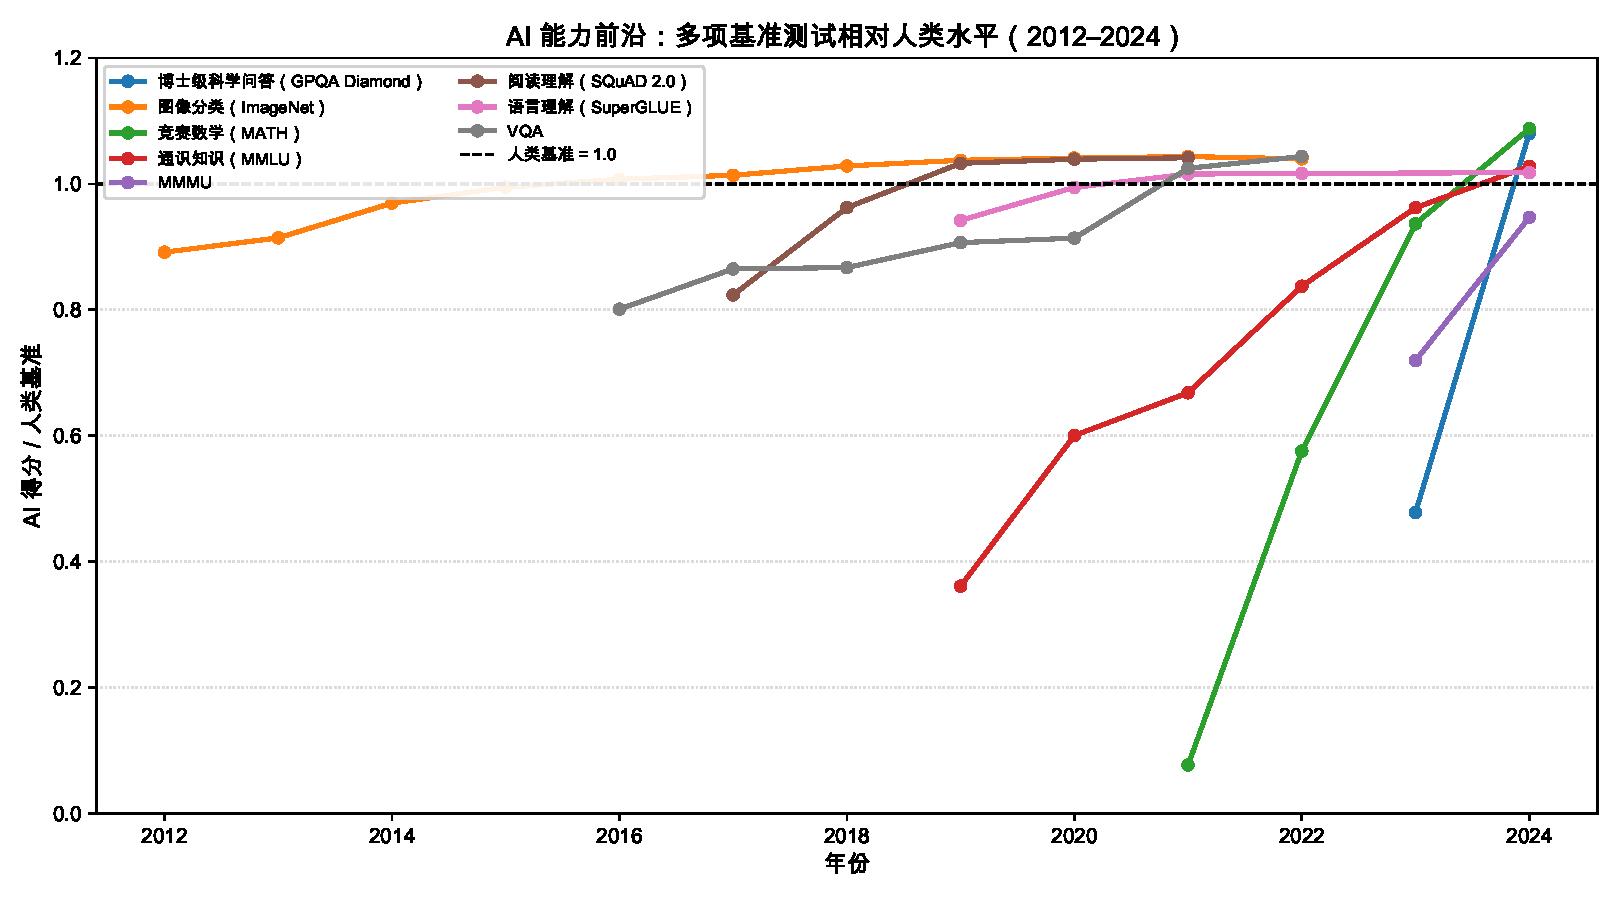
\includegraphics[width=12cm,totalheight=5.0cm,keepaspectratio]{ch10_ai_performance}
\par\end{center}
\vspace{-1mm}
{\scriptsize AI benchmark performance, 2012--2024: AI now \emph{exceeds} human baselines on most standard tasks. Source: Stanford AI Index; \bookAIeconIntro.}
\begin{itemize}\footnotesize
\item For economists, the headline is not ``AI beats humans on benchmarks'' but that a \emph{general-purpose cognitive input} is now cheap, fast, and improving --- the kind of shock that belongs in a growth or labor model.
\end{itemize}
\end{frame}

\begin{frame}{\ldots And Getting Cheaper}
\begin{center}
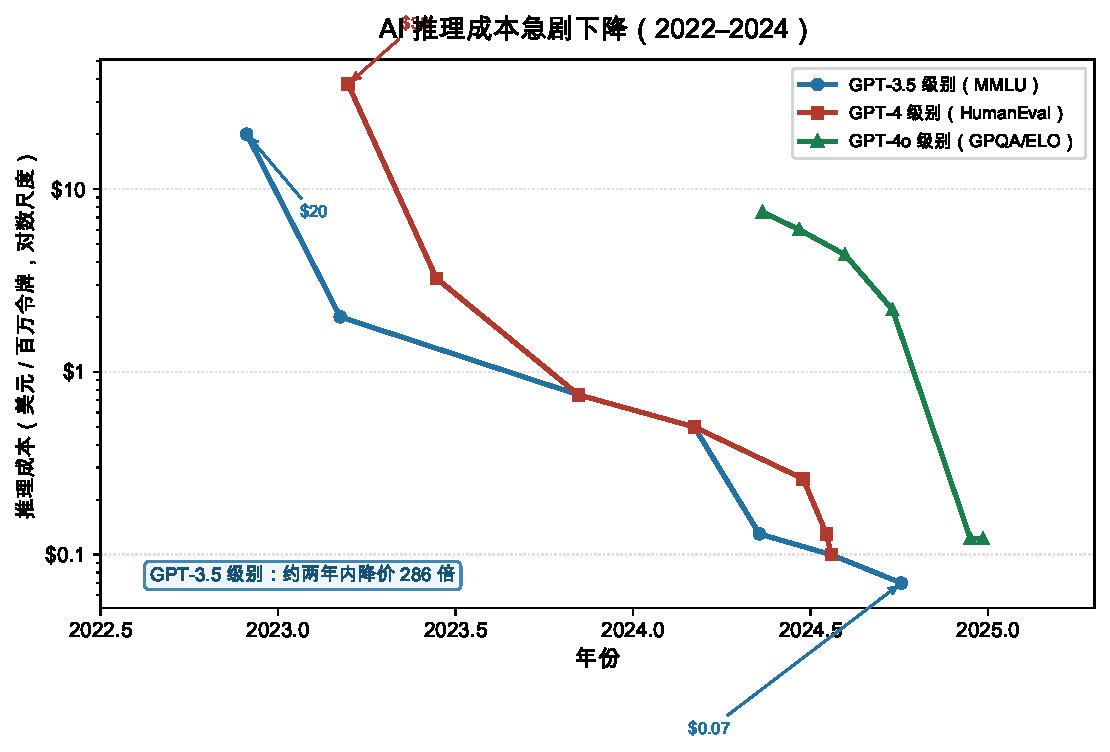
\includegraphics[width=12cm,totalheight=5.0cm,keepaspectratio]{ai_cost_performance}
\par\end{center}
\vspace{-1mm}
{\scriptsize Inference cost has fallen $\sim$280$\times$ in three years; capabilities have compounded simultaneously. Source: \bookAIeconIntro.}
\begin{itemize}\footnotesize
\item The economically relevant variable is the \emph{price of cognition}. When the marginal cost of a competent draft, proof sketch, or block of code falls by orders of magnitude, the optimal mix of human and machine effort in every task shifts.
\end{itemize}
\end{frame}

\begin{frame}{Adoption at Historic Speed}
\begin{center}
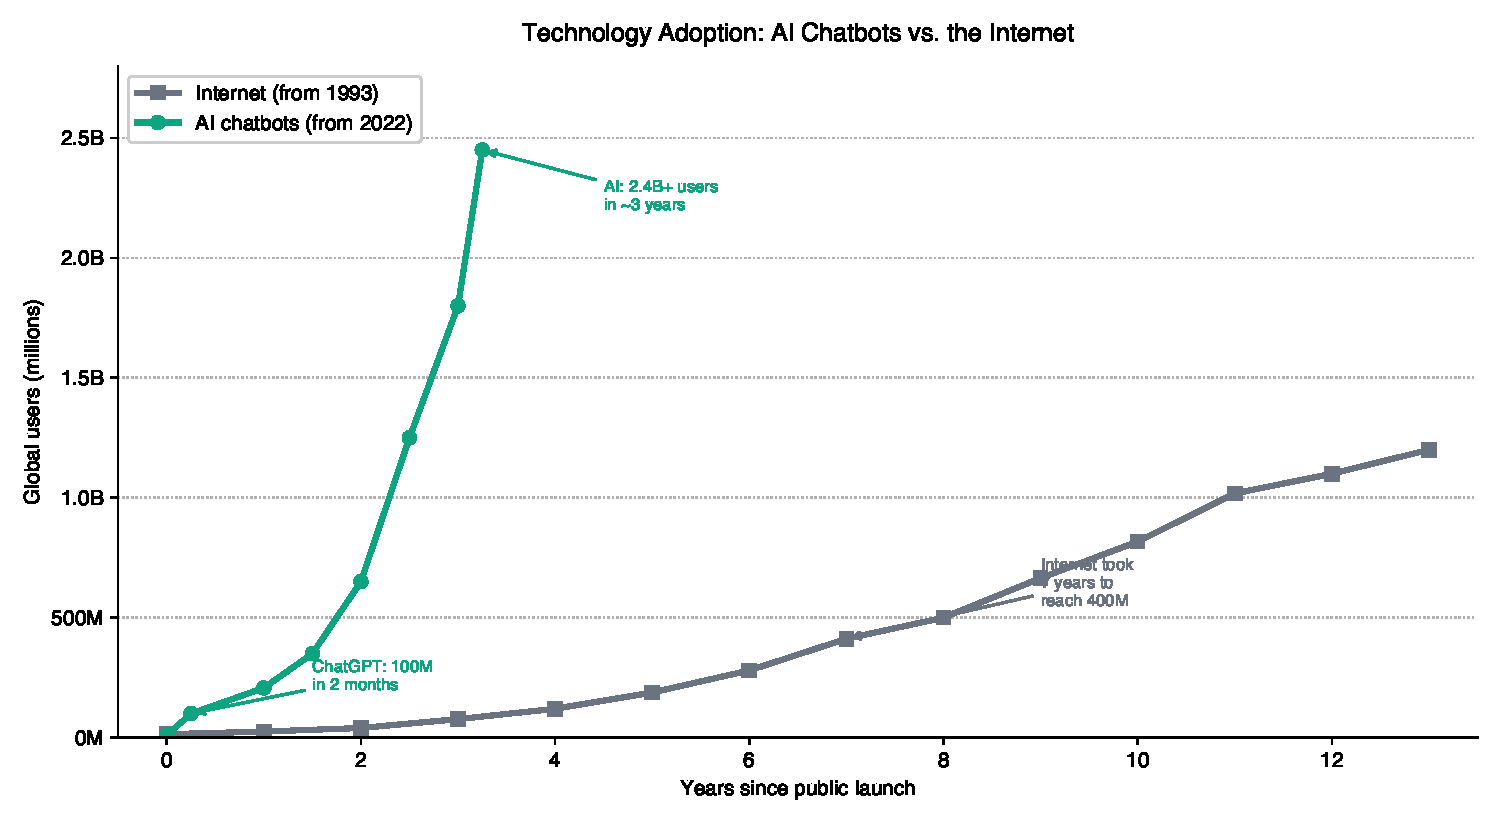
\includegraphics[width=12cm,totalheight=5.0cm,keepaspectratio]{ai_platform_adoption}
\par\end{center}
\vspace{-1mm}
{\scriptsize ChatGPT reached 100M users in two months --- the fastest consumer technology adoption in history. Source: \bookAIeconIntro.}
\begin{itemize}\footnotesize
\item Diffusion this fast is rare: most general-purpose technologies took decades to reach households. The speed compresses the window in which firms, workers, and policy adjust.
\end{itemize}
\end{frame}

\begin{frame}{Diffusion into Firms, and a Multipolar Frontier}
\begin{center}
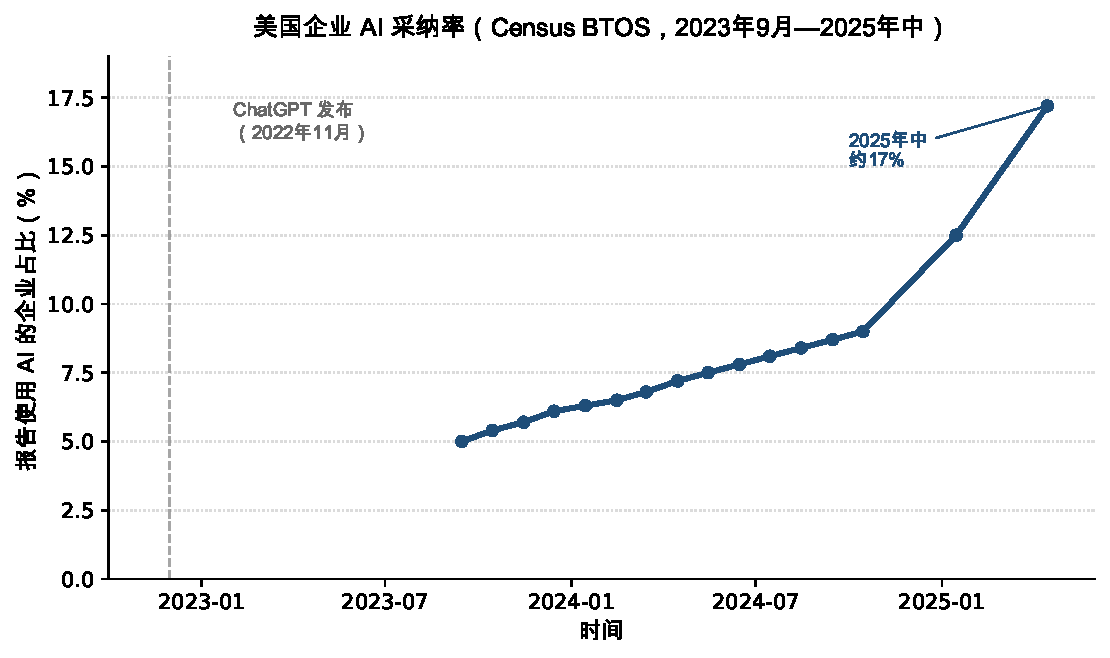
\includegraphics[width=11cm,totalheight=3.6cm,keepaspectratio]{ch10_btos_ai_adoption}
\par\end{center}
\vspace{-1mm}
{\scriptsize U.S.\ business AI adoption (Census Bureau BTOS), 2023--2024: rapid diffusion across sectors and firm sizes. Source: \bookAIeconIntro.}
\begin{itemize}\footnotesize
\item \textbf{Multipolar frontier (as of early 2026):} U.S.\ labs (OpenAI, Anthropic, Google DeepMind) sit alongside strong open-weight and Chinese models (DeepSeek, Qwen) that have closed much of the capability gap and cut the cost of academic experimentation.
\item \textbf{Investment, hedged:} capital flooding in is the macro story --- and \emph{reported, as of early 2026}, several frontier labs (e.g.\ Anthropic, OpenAI) and Chinese players such as MiniMax are discussed as potential IPO candidates. Treat all such figures as a moving target.
\end{itemize}
\end{frame}

\begin{frame}{Why Economists Should Care: AI as a General-Purpose Technology}
\begin{itemize}
\item \textbf{The GPT thesis.} Like the steam engine, electricity, and information technology, AI looks like a \emph{general-purpose technology}: it is
\begin{itemize}
    \item \emph{pervasive} --- usable across essentially every sector and task;
    \item \emph{improving} --- getting cheaper and more capable on a steep curve;
    \item \emph{innovation-spawning} --- it complements and triggers new methods, products, and business models.
\end{itemize}
\medskip
\item That profile is exactly what growth theory studies. So AI is not only a computer-science topic --- it is an object for \textbf{growth, labor, and productivity} analysis.
\end{itemize}
\vfill
\begin{takeawaybox}
\footnotesize
\textbf{Framing for the course.} We treat AI as an economic input --- a new kind of capital --- and ask the economist's questions: what does it substitute for, what does it complement, how is it priced, and how does it show up in output and the distribution of income?
\end{takeawaybox}
\end{frame}

\begin{frame}{What Makes a Technology ``General-Purpose''?}
\begin{itemize}
\item \textbf{The test (Bresnahan \& Trajtenberg, 1995).} A general-purpose technology (GPT) is (i) \emph{pervasive} across sectors, (ii) \emph{improves} steadily over time, and (iii) spawns \emph{complementary innovations} that compound its effect.
\medskip
\item \textbf{The ones that delivered} --- reshaping growth over \emph{decades}:
\begin{itemize}
    \item the \emph{steam engine}; \emph{electricity} (the dynamo); the \emph{internal-combustion engine};
    \item the \emph{semiconductor / computer}; the \emph{internet}.
\end{itemize}
\end{itemize}
\vfill
\begin{conceptbox}
\footnotesize
\textbf{Complementarities take time.} David (1990), ``The Dynamo and the Computer'': factories needed $\sim$40 years to redesign around electricity before the productivity gains showed up. GPT payoffs \emph{lag} the invention --- the same J-curve we should expect for AI.
\end{conceptbox}
\end{frame}

\begin{frame}{\ldots But Not Everything Hyped Is a GPT}
\textbf{Many technologies were announced as transformational --- even ``general-purpose'' --- and never delivered economy-wide:}
\smallskip
\begin{itemize}\footnotesize
    \item \textbf{Nuclear fission power} --- ``too cheap to meter'' (1954); stalled on cost, safety, and regulation.
    \item \textbf{Supersonic passenger flight} (Concorde) --- retired; a niche, not a transport revolution.
    \item \textbf{3D printing} --- valuable for prototyping; not the predicted manufacturing revolution.
    \item \textbf{The Segway} --- hyped to ``redesign cities''; a commercial flop.
    \item \textbf{Web3 / blockchain} --- promised to rewire finance and the web; limited diffusion so far.
    \item \emph{\ldots and the perennial ``a decade away'' list: the hydrogen economy, VR / the metaverse, hyperloop.}
\end{itemize}
\vfill
\begin{takeawaybox}
\footnotesize
\textbf{GPT status is an \emph{ex-post} verdict, not a press release.} The honest question for AI is \emph{which bucket} it lands in --- a genuinely open, empirical question, and one reason this course treats it carefully rather than triumphantly.
\end{takeawaybox}
\end{frame}

%=============================================================================
\section{AI as Cognitive Capital}

\sectiondivider{AI as Cognitive Capital}{Non-rival, self-replicating, scalable: a new factor of production}

% REUSE (verbatim) from Lec02_T2_Cognitive_Capital_Roadmap.tex, lines 32-64.
\begin{frame}{AI as Cognitive Capital: The Economic Framing}
\begin{center}
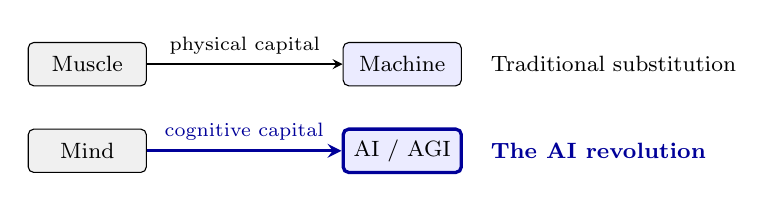
\begin{tikzpicture}[
    every node/.style={font=\footnotesize},
    labor/.style={draw, rounded corners=2pt, minimum width=1.5cm, minimum height=0.55cm, align=center, fill=gray!12},
    capital/.style={draw, rounded corners=2pt, minimum width=1.5cm, minimum height=0.55cm, align=center, fill=blue!8},
    flow/.style={->, >=stealth, semithick},
]
\node[labor] (muscle) at (0, 0.6) {Muscle};
\node[capital] (machine) at (4.0, 0.6) {Machine};
\draw[flow] (muscle) -- node[above, font=\scriptsize]{physical capital} (machine);
\node[font=\footnotesize, anchor=west] at (5.0, 0.6) {Traditional substitution};
\node[labor] (mind) at (0, -0.5) {Mind};
\node[capital, very thick, draw=blue!60!black] (ai) at (4.0, -0.5) {AI / AGI};
\draw[flow, blue!60!black, very thick] (mind) -- node[above, font=\scriptsize, blue!60!black]{cognitive capital} (ai);
\node[font=\footnotesize\bfseries, blue!60!black, anchor=west] at (5.0, -0.5) {The AI revolution};
\end{tikzpicture}
\end{center}

\smallskip
\begin{itemize}
\item \textbf{What Makes AI Different from Other Capital?}
\begin{enumerate}
    \item \emph{Scalability:} Copy model weights instantly; serve $10^6$ users in parallel
    \item \emph{Replication:} Training a new human takes 20 years; training a new AI takes days
    \item \emph{Non-rivalry:} Unlike physical capital, AI can be used simultaneously
    \item \emph{Recursion:} AI can generate data and code to improve itself
\end{enumerate}

\medskip
\item \textbf{Implication:} Cognitive labor transforms from a biological constraint into a scalable, manufacturable capital good.
\end{itemize}
\end{frame}

% Split (was one crowded frame reused from Lec02_T2 lines 66-106) into three.
\begin{frame}{The Economics of AI Adoption: Task-Level Production}
\begin{itemize}
\item Think of output as produced task by task. Within task $i$, human cognitive labor $h_i$ and AI inference $m_i$ combine with elasticity of substitution $\sigma_i$:
\[
H_i = \left[ \varphi_i\, h_i^{\frac{\sigma_i-1}{\sigma_i}} + (1-\varphi_i)\, (\theta_i m_i)^{\frac{\sigma_i-1}{\sigma_i}} \right]^{\frac{\sigma_i}{\sigma_i-1}}
\]
\item $\theta_i$ = AI \emph{capability} on task $i$; \; $\varphi_i$ = weight on human labor; \; $\sigma_i$ = how easily AI substitutes for the human.
\medskip
\item \textbf{Reading it.} As $\theta_i$ rises and AI's price falls, the cost-minimizing mix tilts toward $m_i$ --- quickly where $\sigma_i$ is high (close substitute), slowly where it is low (complement).
\end{itemize}
\vfill
\begin{conceptbox}\footnotesize
The two unobservables here --- the capability index $\theta_i$ and the adoption margin (next slide) --- are exactly what Topic 1.2's measurement example tries to recover from data.
\end{conceptbox}
\end{frame}

\begin{frame}{When Is a Task Automated? The Adoption Margin}
\begin{itemize}
\item Task $i$ is automated when the value of automating exceeds the upfront cost:
\[
E_i(t) = 1 \iff V_i(t) \geq C_i^{\text{upfront}}(t)
\]
\medskip
\item \textbf{Value} scales with the wage saved, the price of inference, and how often the task runs:
\[
V_i(t) = \frac{(w_i - p_t) \cdot \text{Scale}_i}{\rho}
\]
where $w_i$ = human wage, $p_t$ = AI inference price, $\rho$ = discount rate.
\medskip
\item \textbf{Cost} is convex in required precision: low-tolerance tasks (surgery, formal proofs, audited accounts) stay expensive to automate even when raw capability is high.
\end{itemize}
\end{frame}

\begin{frame}{Adoption Follows an S-Curve}
\begin{itemize}
\item Putting the margin in motion: as $p_t$ falls and $\theta_i$ rises, tasks cross the threshold \emph{in order} --- easy, high-scale tasks first; hard or low-scale tasks much later.
\item The result is the familiar \emph{S-curve} of diffusion, and a long tail of tasks that resist automation.
\end{itemize}
\vspace{1mm}
\begin{center}
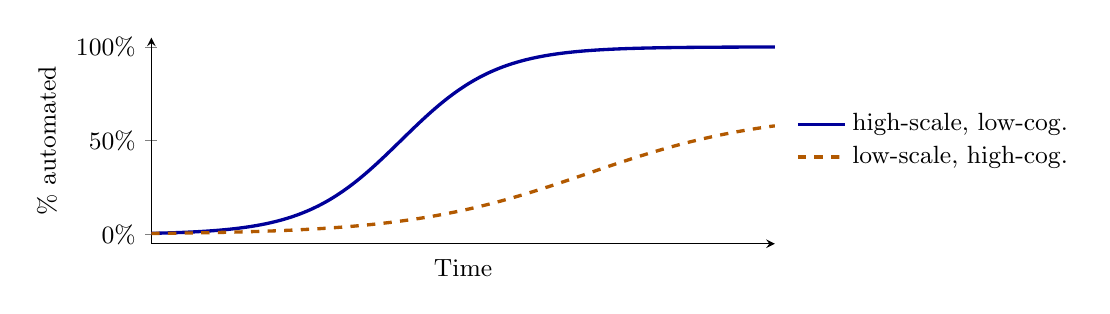
\begin{tikzpicture}
\begin{axis}[
    width=9.5cm, height=4.2cm,
    xlabel={Time}, ylabel={\% automated},
    xtick=\empty, ytick={0, 50, 100}, yticklabels={0\%, 50\%, 100\%},
    ymin=-5, ymax=105, xmin=0, xmax=10,
    axis lines=left,
    tick label style={font=\small},
    label style={font=\small},
    legend style={font=\small, draw=none, at={(1.02,0.5)}, anchor=west, fill=none},
    legend cell align=left,
]
\addplot[blue!60!black, very thick, smooth, samples=60, domain=0:10] {100/(1+exp(-1.3*(x-4)))};
\addlegendentry{high-scale, low-cog.}
\addplot[orange!70!black, very thick, dashed, smooth, samples=60, domain=0:10] {65/(1+exp(-0.7*(x-7)))};
\addlegendentry{low-scale, high-cog.}
\end{axis}
\end{tikzpicture}
\end{center}
\end{frame}

\begin{frame}{Intangible, Non-Rival Capital --- and a Measurement Gap}
\begin{itemize}
\item AI capital is \textbf{intangible} (model weights, prompts, pipelines, skills) and \textbf{non-rival} (the same model serves many users at once) --- unlike a rival machine that one plant uses at a time.
\medskip
\item National accounts were built to measure \emph{tangible, rival} capital. They struggle with software, data, and now AI: much of the value shows up as better decisions, faster code, and improved service quality that GDP captures poorly.
\medskip
\item This is the modern face of the \emph{Solow productivity paradox}: ``you can see the AI age everywhere but in the productivity statistics'' --- partly a measurement problem, partly a diffusion-lag problem.
\end{itemize}
\vfill
\begin{conceptbox}
\footnotesize
\textbf{Why it matters.} If AI is non-rival cognitive capital that the accounts mismeasure, then standard growth and productivity numbers are a \emph{lower bound} on its effect --- and measuring it correctly is itself a research agenda (we build toward one in Topic 1.2).
\end{conceptbox}
\end{frame}

%=============================================================================
\section{Where AI Enters the Economy}

\sectiondivider{Where AI Enters the Economy}{Three channels into growth --- and why the statistics may understate all of them}

\begin{frame}{Three Channels: How AI Enters Growth}
\begin{center}
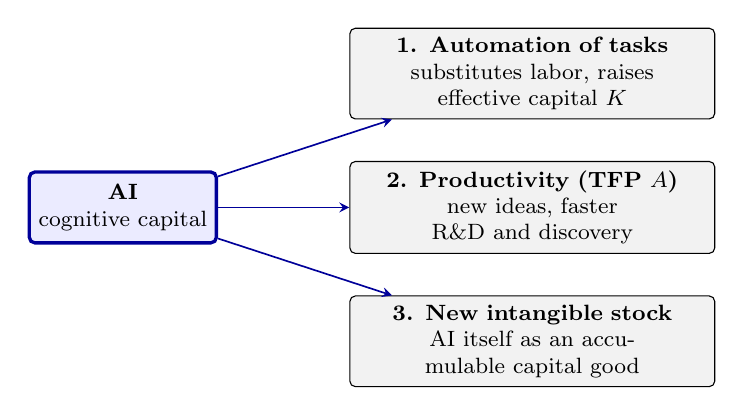
\begin{tikzpicture}[
    every node/.style={font=\footnotesize},
    ai/.style={draw, very thick, draw=blue!60!black, fill=blue!8, rounded corners=2pt, minimum width=1.8cm, minimum height=0.9cm, align=center},
    ch/.style={draw, rounded corners=2pt, fill=gray!10, minimum width=4.6cm, minimum height=0.95cm, align=center, text width=4.4cm},
    flow/.style={->, >=stealth, semithick, blue!60!black},
]
\node[ai] (ai) at (0, 0) {\textbf{AI}\\cognitive capital};
\node[ch] (k) at (5.2, 1.7) {\textbf{1. Automation of tasks}\\substitutes labor, raises effective capital $K$};
\node[ch] (a) at (5.2, 0.0) {\textbf{2. Productivity (TFP $A$)}\\new ideas, faster R\&D and discovery};
\node[ch] (s) at (5.2, -1.7) {\textbf{3. New intangible stock}\\AI itself as an accumulable capital good};
\draw[flow] (ai) -- (k);
\draw[flow] (ai) -- (a);
\draw[flow] (ai) -- (s);
\end{tikzpicture}
\end{center}
\vspace{1mm}
\begin{itemize}\footnotesize
\item The three channels map onto the three terms of a growth-accounting identity --- which we make precise next.
\end{itemize}
\end{frame}

\begin{frame}{A Light Growth-Accounting Lens}
\begin{itemize}
\item Standard Solow decomposition of output growth:
\[
\Delta\ln Y \;=\; \alpha\,\Delta\ln K \;+\; (1-\alpha)\,\Delta\ln L \;+\; \Delta\ln A
\]
where $\alpha$ is capital's share, and $\Delta\ln A$ is the Solow residual (TFP).
\medskip
\item \textbf{Where AI shows up:}
\begin{itemize}
    \item in $\Delta\ln K$ --- automation and capital deepening (Channel 1);
    \item in $\Delta\ln A$ --- AI as an ideas / TFP shifter (Channel 2);
    \item as a \emph{new intangible capital input} that the standard $K$ measure omits (Channel 3).
\end{itemize}
\medskip
\item This is deliberately a \emph{lens}, not a model. The deep dynamic-programming and growth foundations --- Bellman equations, optimal growth, heterogeneous agents --- arrive in Lec.\ 4 and Lec.\ 6.
\end{itemize}
\end{frame}

\begin{frame}{Task Gains Don't Auto-Sum to Macro TFP}
\begin{itemize}
\item It is tempting to add up task-level productivity gains into an aggregate number. But aggregation is weighted and bottlenecked:
\[
\Delta A_{\text{macro}} \;\approx\; \sum_i \omega_i\,\Delta a_i
\]
where $\omega_i$ is task $i$'s share and $\Delta a_i$ its productivity gain.
\medskip
\item \textbf{Bottlenecks dominate.} If a few hard-to-automate tasks ($\Delta a_i \approx 0$) carry large weight, they cap the aggregate (a Baumol / weakest-link logic): automating the easy 80\% barely moves macro TFP if the binding 20\% does not budge.
\end{itemize}
\vfill
\begin{cautionbox}
\footnotesize
\textbf{A sober benchmark.} Acemoglu (2024), \emph{The Simple Macroeconomics of AI}, estimates no more than $\sim$0.66\% TFP gain over 10 years (possibly $\sim$0.53\%), because only $\sim$4.6\% of tasks are currently exposed to AI automation. Big task-level wins, modest measured-macro effect --- so far.
\end{cautionbox}
\end{frame}

\begin{frame}{Bridge: From Framing to Practice}
\begin{itemize}
\item \textbf{Where we are.} AI is cheap, fast, diffusing, and best understood as \emph{non-rival cognitive capital} --- a general-purpose technology that reshapes growth and labor through three channels, with effects that today's statistics likely understate.
\end{itemize}
\medskip
\begin{cautionbox}\footnotesize
\textbf{Read this lecture as a moving snapshot.} The AI frontier is changing on a timescale of \emph{months} --- capabilities, costs, market structure, and policy are all in flux.
The economics of AI is an \textbf{active, unsettled research area}: our understanding (and many of the numbers here) will keep evolving quickly. Treat results as current best estimates, not settled facts.
\end{cautionbox}
\vfill
\begin{takeawaybox}
\footnotesize
\textbf{Next (1.2):} leave the framing behind and watch AI \emph{actually do} frontier economic research --- two live case studies and a measurement example.
\emph{Lecture 2} (``What is AI'') then opens the toolbox: the technique families (ML / DL / RL / LLM / agentic) and where AI is powerful \emph{but bounded}.
\end{takeawaybox}
\vspace{0.15cm}
\begin{center}
\footnotesize\textit{Arc: \textbf{1.1 FRAME} (cognitive capital) $\;\to\;$ 1.2 PROOF (AI doing research) $\;\to\;$ 1.3 PRACTICE (course $+$ capstone).}
\end{center}
\end{frame}

\end{document}
